\section{Introduction}
The focus of the previous Chapter was to understand how visual experience during development modifies behaviour and developing spontaneous activity within the tectum. To do this, zebrafish larvae were raised either under normal laboratory rearing conditions or in enriched conditions, where a petri dish was placed over a bed of gravel. These changes in the visual environment were found to have two main effects: 

\begin{enumerate}
    \item  GR fish were found to consume more prey than NR fish when hunting over the GB but not a plain WB. Importantly, this was not due to the NR fish eating less food when hunting over the GB as they consume a similar number of prey in either background. This suggests that during development the GR fish have learnt to exploit a feature/features of the GB and this facilitates them in eating more prey. 
    \item Spontaneously active tectal assemblies in GR fish appear to follow a completely different developmental trajectory to NR between 5 - 7 \gls{dpf}. This resulted in the 7 \gls{dpf} GR fish having neural assemblies that were larger, more active and less synchronous than those seen in the tectum of NR fish. 
\end{enumerate}

While these changes in spontaneous activity demonstrate that EE shapes the development of the tectum, it is difficult to relate changes in the structure and dynamics of spontaneous activity to the changes in hunting behaviour.

Hunting in zebrafish consists of multiple different steps, each of which could be modified by enrichment, to alter prey consumption. First, a fish has to detect a potential target from its surroundings and make a decision on whether it is worth pursuing. Then, if hunting is initiated, the fish converges its eyes and orientates itself towards the prey using a characteristic J-turn, where the tip of the tail bends unilaterally towards the stimulus. This is then followed by a series of minor adjustments in heading direction, as the fish tracks the prey, and ends with a final high velocity strike at the prey (\cite{Budick2000LocomotorCapture}; \cite{Gahtan2005}; \cite{Patterson2013}; \cite{McElligott2005PreyControl}). Based on this sequence of events, there are two potential ways that enriched fish may be using the GB to increase their prey consumption: 1) The GB may help enriched fish in initially detecting prey -  this would allow the fish to engage in more hunting routines thus increasing prey consumption. Or 2) the GB helps enriched fish to better locate their prey, leading to more accurate turns in the hunting sequence, increasing hunting efficiency, although both of these possibilities may not be mutually exclusive.

One possible way that these hypotheses could occur is that the gravel background could contextually modulate the population response in the tectum, altering the perception of prey. This is interesting because the contextual modulation of neural responses when viewing visual scenes is already a well known phenomenon (\cite{Spillmann2015BeyondStimuli}). In the simplest case contextual modulation has previously been shown to alter the receptive field properties of single neurons through center-surround modulation. This is where responses to visual stimuli positioned in the center of the receptive field can be either facilitated, or suppressed, by presenting different visual features such as changes in luminance, contrast or more complex spatiotemporal properties to the surrounding visual space (\cite{Krause2014ContextualCortex}; \cite{Sun2002ContextualPigeons}; \cite{Huang2019NeuralCircuit}). Such modulation has been shown to be most pronounced when the surrounding stimuli mimic the statistics of natural visual scenes rather than those that have been phase scrambled (\cite{Guo2005Centre-surroundCortex}). This has lead to the notion that circuitry in the visual system may utilise contextual modulation as a mechanism to segment natural scenes, allowing salient features to be identified, potentially contributing to "pop-out" phenomena. Furthermore, neurons in the visual system of dark reared animals have been found to exhibit reduced center-surround modulation, suggesting that the structure of of natural scenes is required to shape this form of contextual modulation  (\cite{Pecka2014Experience-DependentScenes}). Therefore it is possible that the responses of neurons in the tecta of GR fish are contextually modulated by the presence of the GB, leading to an enhanced ability to detect or localise the prey and that this ability is acquired through their exposure to the gravel during development. 

To investigate this hypothesis it is necessary to image activity in the tectum when GR and NR fish are viewing prey over the textured and non-textured backgrounds. Whilst imaging visually evoked tectal activity is difficult in freely moving fish, a number of studies have shown that hunting behaviours can be elicited in head fixed preparations, by projecting artificial stimuli onto a screen (\cite{Bianco2011}; \cite{Trivedi2013VisuallyCapture}; \cite{Semmelhack2014}; \cite{Bianco2015}; \cite{Jouary2016ALarvae}). In these preparations eye convergence and J-turns can be elicited by small moving dots of 1$^{\circ}$ to 10$^{\circ}$ in size (\cite{Bianco2015}; \cite{Semmelhack2014}). The size of these dots corresponds to the size of prey on the retina when hunting is initiated in freely swimming fish. This allows for both neural activity in the tectum and the behavioural output to be monitored in a virtual reality hunting assay.

One way to study how much information is encoded about a particular stimulus is to decode certain characteristics from visually evoked activity within the brain (\cite{Glaser2017MachineDecoding}); \cite{Quaglio2017}). In virtual hunting assays prey-like stimuli elicit the activation of spatially compact tectal assemblies (\cite{Bianco2015}; \cite{Romano2015}; \cite{Avitan2016}; \cite{Avitan2019}). Each of the constituent neurons by themselves can be unreliable and have a spatial tuning profiles that are broader than the size of the prey (40$^{\circ}$), leading to poor decoding of stimulus location (\cite{Niell2005FunctionalTectum}; \cite{Romano2015}; \cite{Avitan2016}). Instead, the combined statistics from multiple neurons can provide a much more accurate prediction of a object's position in visual space,  suggesting a population code for stimulus location (\cite{Averbeck2006NeuralComputation}; \cite{Avitan2019}). As a result, the position of very closely spaced stimuli, which producing overlapping patterns of activation in the tectum, can be accurately predicted with simple linear decoding methods (\cite{Avitan2016}; \cite{Avitan2019}). Recently, decoding performance has been used to understand how the ability of the tectum to localise prey changes during development (\cite{Avitan2019}). This work revealed that the sensory representation of prey location becomes more refined over the course of development. Furthermore, not only did this refinement correlate with hunting performance across developmental stages but high decoding performance from the tecta of individual fish accurately predicted their hunting performance. This demonstrates that decoding can be used as a biologically relevant tool to study the neural correlates of changes in hunting performance.

In this chapter I outline a virtual reality hunting experiment designed to understand how the sensory representation of prey-like stimuli in the enriched fish is altered. In this experiment fish are presented with artificial prey at different locations in the visual scene which are separated by a few degrees in visual azimuth. These stimuli evoke overlapping activation patterns in tectal neurons. Importantly the larvae view these stimuli over either an untextured background (grey screen) or textured background (a picture of gravel) while both their tectal activity and tail movements are monitored. The aim of this experiment is to understand how the sensory representation of prey location changes when prey is viewed over textured/non-textured backgrounds, by decoding prey location from the tectum. Based on the results from the hunting assay in Chapter 4, the hypothesis is that GR would show an increased decoding performance when viewing  prey over the textured background whereas the NR would not. Finally, monitoring the fish's tail movements allows for the ability of these different stimuli to induce behaviour to be examined.



\section{Results}
\subsection{The virtual reality hunting assay}
To understand how EE is shaping the sensory representation of prey-like stimuli within the tectum we performed a virtual reality hunting assay which was  designed to mimic features of the hunting assay presented in \textbf{Chapter 4}. To do this GR or NR zebrafish larvae expressing \textif{nls-GCaMP6s} were head fixed at 7 \gls{dpf} in agarose in a cylindrical imaging chamber with their right eye facing a semicircular screen that was covered in a diffusive filter (GR: n = 3, NR: n = 1). Agarose was cut away from both the right eye and the tail, allowing for an unobstructed view of the screen and free movement of the tail. The two-photon microscope objective was positioned above the head of the fish allowing for volumetric imaging of tectum (see \textbf{Materials and methods}). This imaging volume was positioned so that the top slice was always 50$\mu$m below the skin covering the dorsal surface of the tectum. Below the fish sat a high speed behavioural camera which recorded the fishes tail movements through the transparent base of the imaging chamber at 450 Hz. This setup allowed for both tectal activity and tail movement to be monitored for 1 hr while visual stimuli were projected onto the screen (\textbf{Figure \ref{fig:R3_F1}A}). 

Visual stimuli were presented in two blocks which differed in their background. In one block the background was a picture of gravel (textured block) and the other it was simply a grey screen (untextured block). Moving black spots (5$^{\circ}$) were presented over these backgrounds at three different locations in visual azimuth and were presented with multiple repeats (see \textbf{Materials and methods}).  These spots are much closer together than the average spatial tuning of tectal neurons and should therefore cause topographically organised but overlapping patterns of activation (\textbf{Figure \ref{fig:R3_F1}B-C}).

\begin{figure}[!ht]
        \captionsetup{}
        \centering
        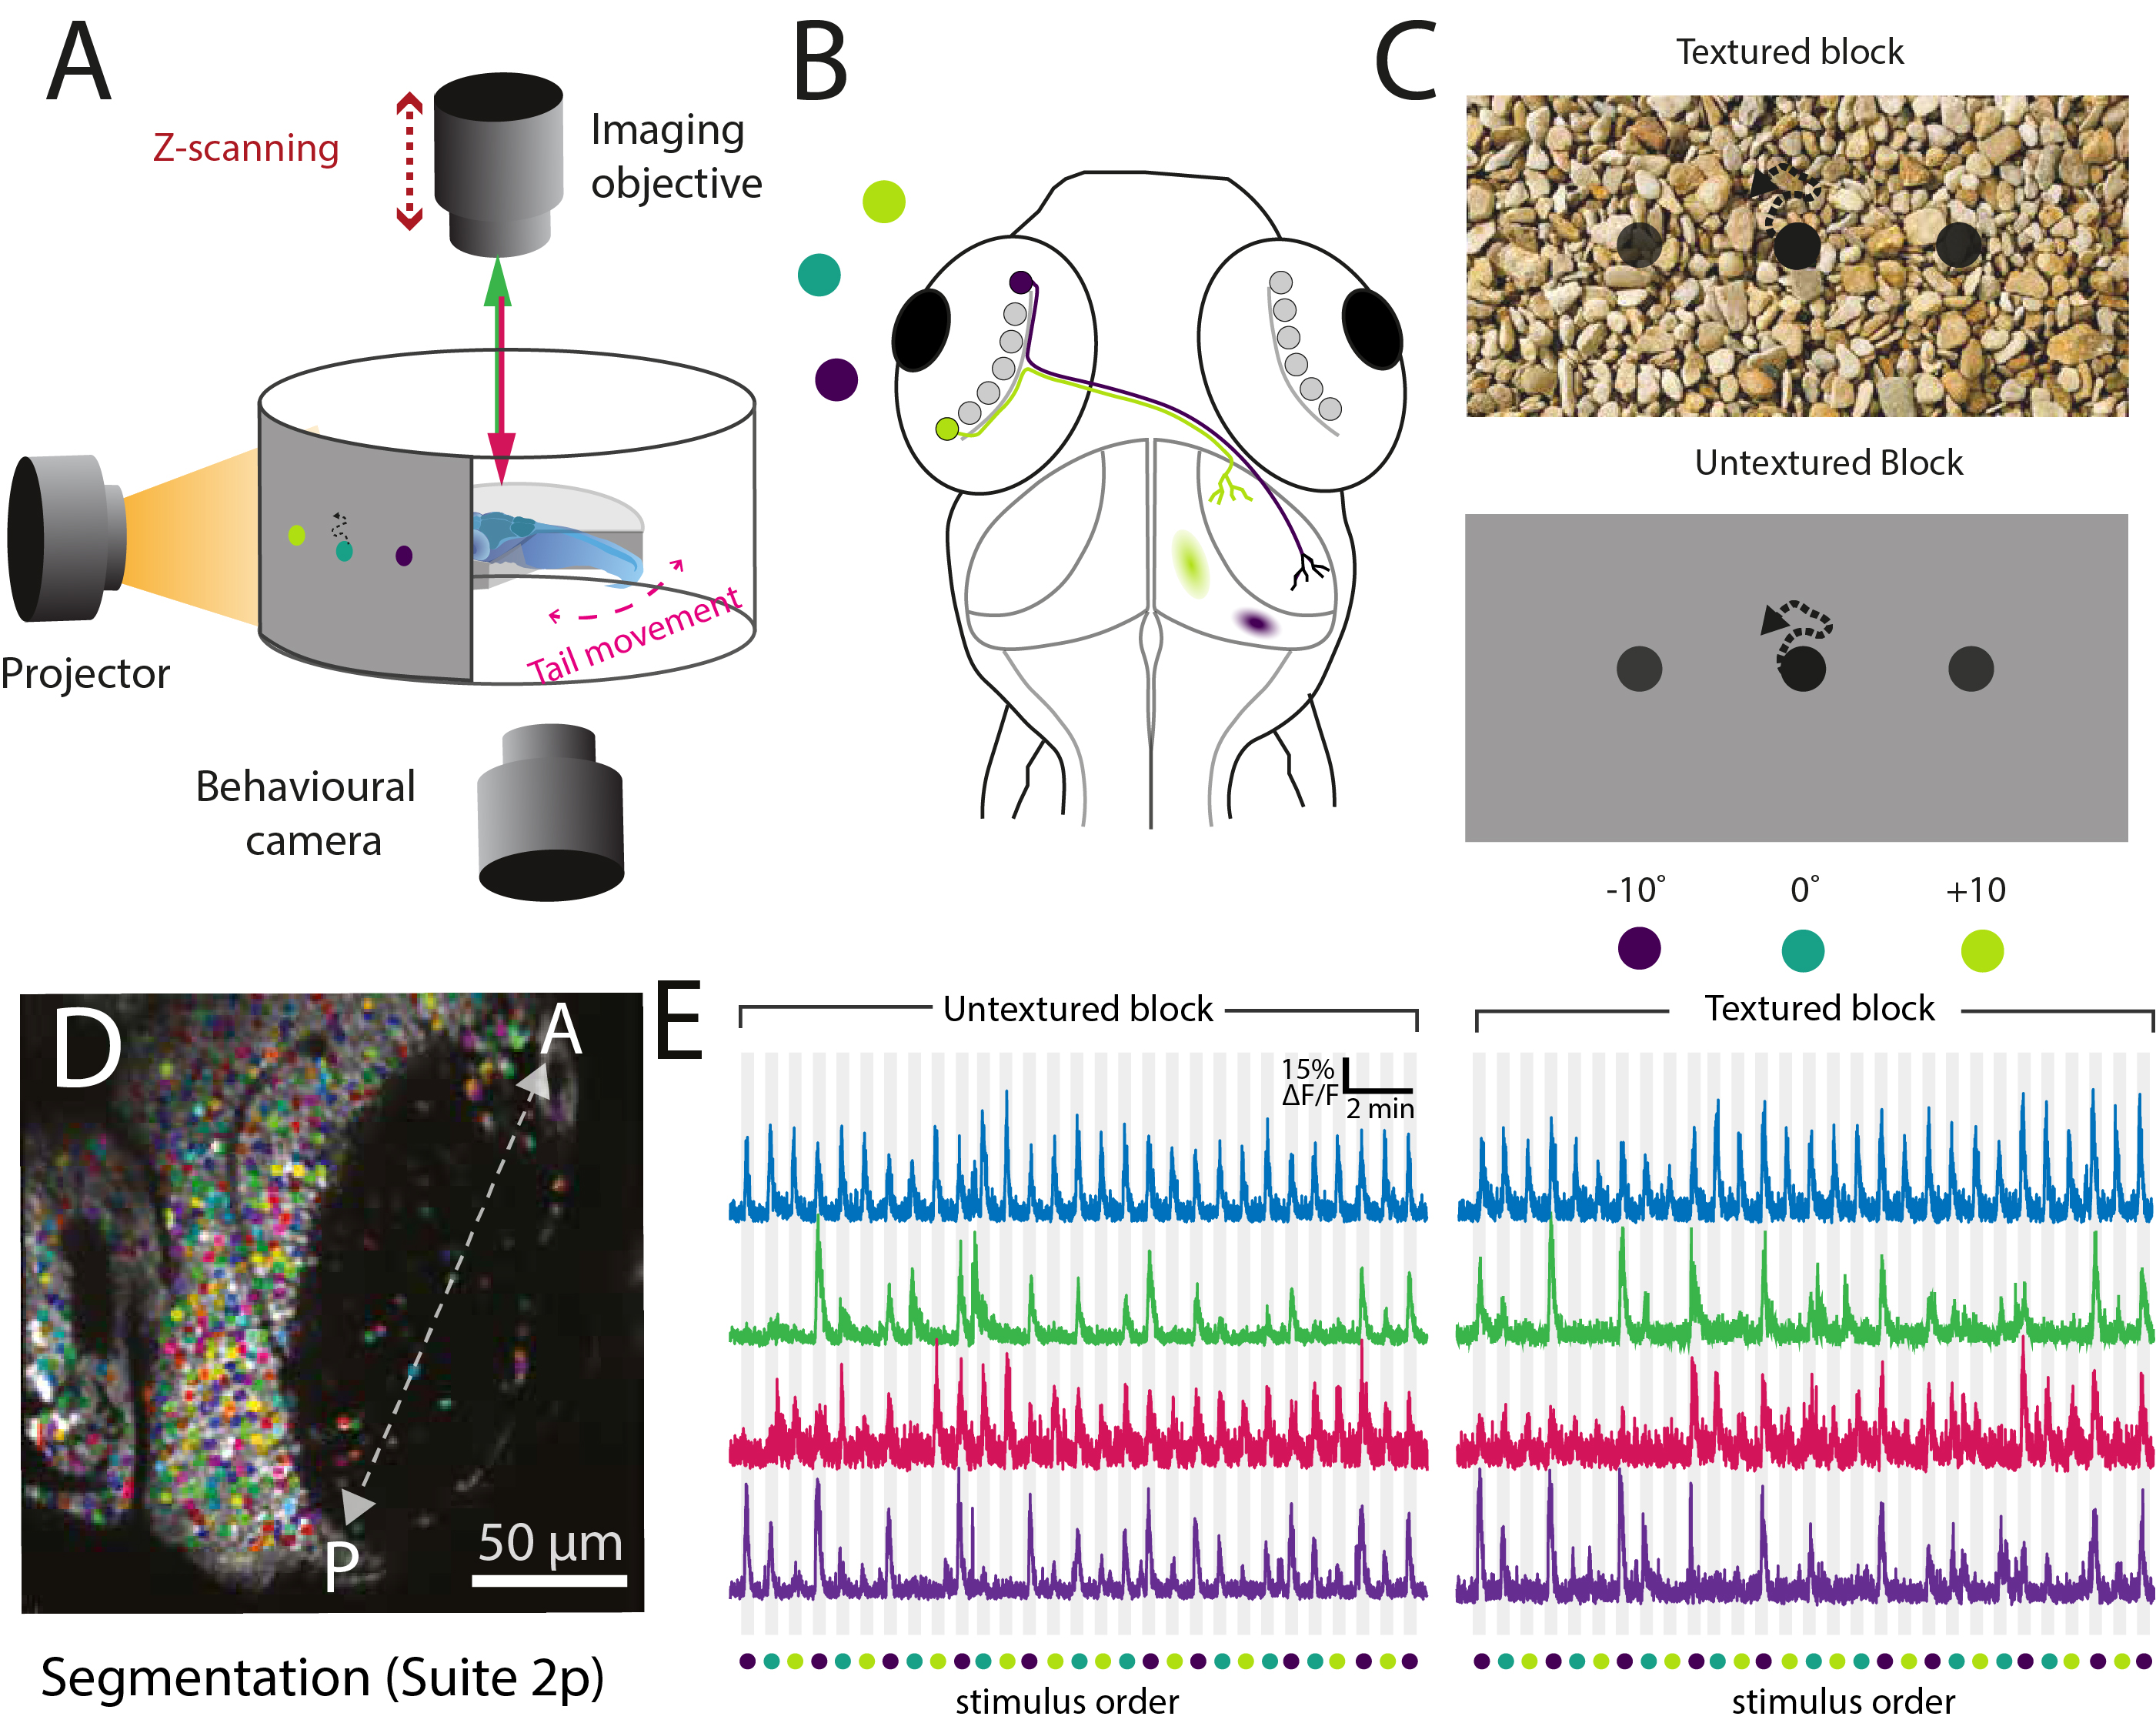
\includegraphics[width =  0.75\paperwidth]{Figures/R3_F1.jpg}
       \caption[\label{fig:R3_F1} \textbf{Virtual reality hunting assay to study tectal responses to prey-like stimuli over different backgrounds.}]{\label{fig:R3_F1} \textbf{Virtual reality hunting assay to study tectal responses to prey-like stimuli over different backgrounds. (A)} In the virtual reality setup a larval zebrafish is head fixed in agarose with one eye facing a screen. Prey-like stimuli are projected onto this screen while monitoring neural activity and tail movements. \textbf{(B)} The optic tectum receives the majority of its input from the contralateral eye via \gls{rgc}s which terminate in a topographic fashion within the tectal neuropil. \gls{rgc}s responding to the rear visual field (purple), with their cell bodies situated in the nasal retina, project to the anterior tectum. \gls{rgc}s responding to the frontal visual field (light green) have their cell bodies situated in the temporal retina and project to the posterior region of the tectum. This retinotopic mapping is reflected in the pattern of activity in the downstream tectal neurons. \textbf{(C)} The visual stimulation occurred in 2 blocks that differed in the background that was projected: a textured block (picture of gravel) and an untextured block (grey screen). In these blocks prey-like stimuli, 5$^{\circ}$ spots moving within a 5$^{\circ}$ neighbourhood (dotted arrow), were presented at different locations within the visual azimuth (-10$^{\circ}$, 0$^{\circ}$, +10$^{\circ}$). Here the stimulus location is denoted by the same coloring as in B. \textbf{(D)} Functional imaging data was aligned and segmented using suite2p, allowing for a large number of cells to be segmented across the tectum. Dotted arrow shows the major axis of the tectal neuropil which is used to sort cells based on the anterior posterior position within the tectum. \textbf{(E)} The $\Delta$F/F of 4 tectal cells responding to stimulus presentations in the untextured and textured blocks. Stimulus presentations (epochs) are shaded in grey and the stimulus location is indicated by the colored dot below with the same coloring scheme as in B and C.
    }
\end{figure}


\subsection{Tectal responses to prey-like stimuli}
Visually evoked functional imaging recordings were aligned and segmented to obtain a fluorescence trace for each neuron. These traces were normalised by calculating their $\Delta$F/F and any inactive cells were removed using a min-max procedure (see \textbf{Materials and methods})(\textbf{Figure \ref{fig:R3_F1}D-E}). Of these neurons only a fraction were found to respond to prey-like stimuli. Some neurons, likely to be related to ongoing activity or behaviour, may negatively impact decoding performance because their activity is sporadic, creating noise for the decoder (\cite{Kahn2015ANeurons}). In order to assess the impact of these cells on decoding performance we distinguished neurons that were responding to the stimulus from those that were not. This was achieved by calculating a \gls{ncc} value for each neuron, which quantified the correlation between the neuron and the stimulus (see \textbf{Materials and methods}). Significant correlations between the neuron and the stimulus were defined as NCC values that were 3 standard deviations more than that expected average NCC value for a randomly firing neuron with the same firing probability. This distinguished neurons that were responding to the stimulus from neurons that were not.

Prior to decoding the visually evoked responses were first inspected to understand if there were any major differences between either the untextured and textured blocks or as a result of rearing condition. \textbf{Figure \ref{fig:R3_F2}A} demonstrates that 
 the NCC measure reliably separates those neurons that are responding to the stimulus consistently (NCC neurons) from those that are not (non-NCC neurons) by displaying them in a raster plot. Consistent with the broad tectal responses previously reported  (\cite{Niell2005FunctionalTectum}; \cite{Romano2015}) each prey-like stimulus for in both untextured and textured blocks elicited visual responses in spatially compact but overlapping populations of neurons. These population responses could be visualised by calculating the mean response for each neuron across repetitions of the same stimulus to generate maps of activity across the tectum (\textbf{Figure \ref{fig:R3_F2}B}). Despite the overlapping responses, rough topographic organisation could still be observed by arranging these mean responses based on their position within the anterior-posterior axis of the tectum. This was achieved by manually fitting a line to the major axis of the tectal neuropil (\textbf{Figure \ref{fig:R3_F1}C}) cells were sorted based on their projection onto this line. The mean response of these sorted cells could then be visualised for stimuli in both the untextured and textures blocks. Neural responses for both blocks showed rough topographic order between the 3 stimuli. 

In Chapter 4 EE was found to alter the number of spontaneously active cells and their response amplitude in the tecta of 7 dpf zebrafish. To investigate if enrichment was also affecting the number of active cells during visual stimulation both the total number of active cells in the tectum and the number of NCC neurons were plotted for NR and GR fish (\textbf{Figure \ref{fig:R3_F2}D}). For two GR fish the number of active cells and NCC neurons was low ($\sim$ 700 total active neurons, $\sim$ 250 NCC neurons) whereas for one GR fish and the NR fish these values were much higher ($\sim$ 1700 total active neurons, $\sim$ 500 NCC neurons). This suggests that there may be high within group variability and no major observable difference between the GR and NR fish in terms of total active neuron or NCC neurons. Next the mean response amplitude for each stimulus in both textured and untextured blocks was calculated for each fish. This was done for NCC neurons and for the total number of active cells in the tectum (\textbf{Figure \ref{fig:R3_F2}E}). While responses for NCC neurons appeared to be slightly higher for fish viewing stimuli over the textured background the NR and GR fish showed similar levels of activity. Whereas the mean amplitude for all cells in the tectum was similar between textured and untextured backgrounds and rearing conditions (\textbf{Figure \ref{fig:R3_F2}F}). While more data is needed to examine this question in more detail these results suggest that there is no major difference in activity when the tectum is responding to stimuli. However, it should be noted that these values represent the mean response to a stimulus presentation and not the mean amplitudes of individual calcium events as calculated in \texChapter 4.

\begin{figure}[!ht]
        \captionsetup{}
        \centering
        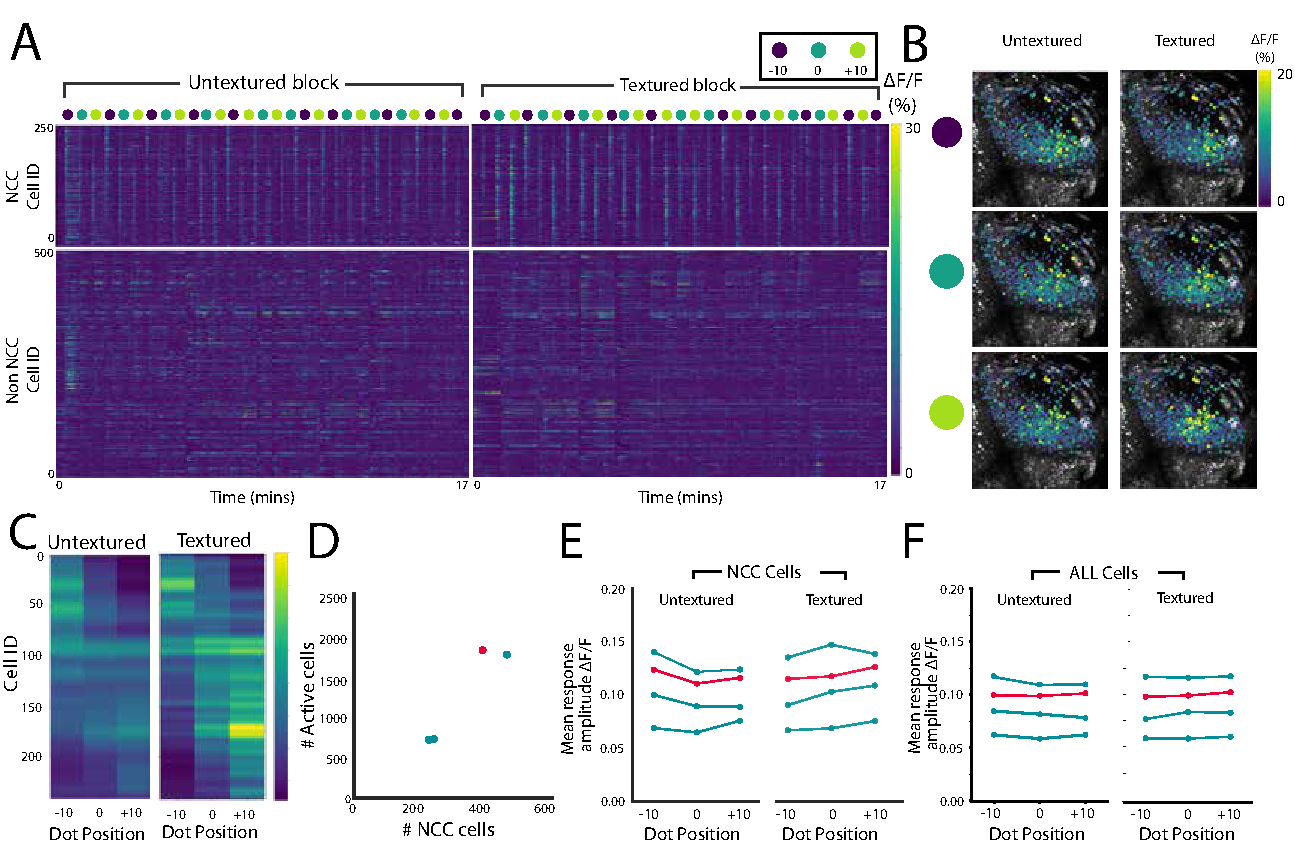
\includegraphics[width =  0.75\paperwidth]{Figures/R3_F2.pdf}
       \caption[\label{fig:R3_F2} \textbf{Tectal responses to prey-like stimuli.}]{\label{fig:R3_F2} \textbf{Tectal responses to prey-like stimuli. (A)} Active tectal cells were sorted into cells that respond to the stimulus consistently (NCC cells) and cells were activity was not stimulus (non-NCC cells). The reason for this is that ongoing tectal activity or activity associated with behaviour may drastically affect decoding performance, making the results difficult to interpret. By plotting both groups of cells in a raster plot revealed that the NCC measure reliably separated out stimulus responsive cells from ongoing tectal activity. \textbf{(B)} Coloring in cells based on their mean response amplitude for a stimulus showed that prey-like stimuli elicited responses from spatially compact populations of neurons. These populations appeared to show a large degree of overlap. \textbf{(C)} Mean responses for each neuron to each stimulus across the two blocks.  Neurons are ordered by their anterior-posterior position within the tectum (top of plots = posterior, bottom = anterior). This shows overlapping activation patterns but also showed rough topographic order between the 3 stimuli. \textbf{(D)} The number responsive neurons (NCC cells) plotted against the total number of active cells in the the tecta of GR (green) and NR fish (red).  \textbf{(E)} The mean response amplitude for NCC cells responding to each of stimulus positions in both untextured and textured blocks. \textbf{(F)} The mean response amplitude for all tectal cells in each fish for each stimulus presentation in both untextured and textured blocks. 
    }
\end{figure}

\subsection{How to decode stimuli for tectal activity?}
Decoding is a useful tool to understand how much information population activity carries about an external stimulus (\cite{Raposo2014ADecision-making}) and has previously been used to understand how this information changes across different brain regions (\cite{vanderMeer2010TripleTask}), experimental conditions (\cite{Glaser2018PopulationCortex}) and disease states (\cite{Weygandt2012FMRIDisorder}). Here we aim to use decoding performance to understand how the ability of the tectum to distinguish between closely positioned stimuli changes as a result of background complexity and rearing condition. To do so a decoder must learn from a given training dataset a function, $f$, that can predict the stimulus identity, $s$, from the visually evoked population response, $r$:

\begin{equation}
    f: r \rightarrow{s}
\end{equation}

where $r = (r_{1}, ..., r_{n})$ is an $n$ dimensional vector where $n$ is the number of cells and $s$  is the different stimulus positions \{-10$^{\circ}$, 0 -10$^{\circ}$, +10$^{\circ}$\}. Therefore decoding performance is likely to be highly influenced by the choice of decoder because this affects how $f$ is determined. Previous attempts to decode the position of a dot like stimulus from tectal activity have suggested that topography based decoders which utilise the retinotopic organisation of the tectum to decode stimulus location perform poorly, due to map imprecision (\cite{Avitan2016}). An alternative strategy is to a linear decoders which do not use information about the neuron's position in the tectum. Instead, these decoders make classifications based on a linear predictor function by combining a set of weights with the feature vector (i.e the population response vector, $r$) (\cite{Avitan2016}; \cite{Avitan2019})

While non-linear decoders, or statistically optimal decoders (such as maximum likelihood decoders), may yield marginal improvements in decoding performance, linear decoders are preferable in this case because: 1) they are more interpretable by indicating a linear separation between classes, 2) have few hyper-parameters that need to be tuned and 3) are simple to implement. Furthermore linear decoders, such as \gls{lda}, have previously been used to investigate how the tectal representation of stimulus location refines across development (\cite{Avitan2019}). In this study decoding performance was found to be predictive of hunting performance, suggesting that changes in linear decoding performance are relevant to understanding the neural basis for changes in behaviour. To ensure that any decoding result was not an artifact of a single decoder and to understand which linear decoder had best performance on my data, I used two different decoders to decode stimulus position from tectal activity: \gls{lda} and \gls{logreg}. The following sections briefly describe the intuition behind these methods (for both decoders the scikit-learn implementation was used -  see \textcolor{blue}{https://scikit-learn.org/} for a detailed description of the methods)


\subsubsection{Linear Discriminant Analysis}
\gls{lda}, like PCA, attempts to find a lower dimensional representation of the data. Unlike PCA, which tries to maximise the variance of the principle components, LDA maximises the distance between between the means $u$ of the classes $c$ to be decoded whilst minimising their within class variance $V$. This process can be simplified by maximising the following equation: 

\begin{equation}
    J(w) = \frac{| u_{c1} - u_{c2}|^{2}}{V_{c1}^{2} + V_{c2}^{2}}
\end{equation}

This gives a lower dimensional projection  of the data  (usually only 1 or 2 dimensions) that maximises the separation between classes making them easier to decode. LDA learns this projection from a training data set and then can apply the learned transformation to new points (test data). LDA then assumes that each of the classes are normally distributed. Using the mean and standard deviation of each class, it calculates the likelihood that the test point came from each of these classes. Therefore if this assumption of being normally distributed is violated the performance of LDA as a decoder can be impacted.

\begin{figure}[!ht]
        \captionsetup{}
        \centering
        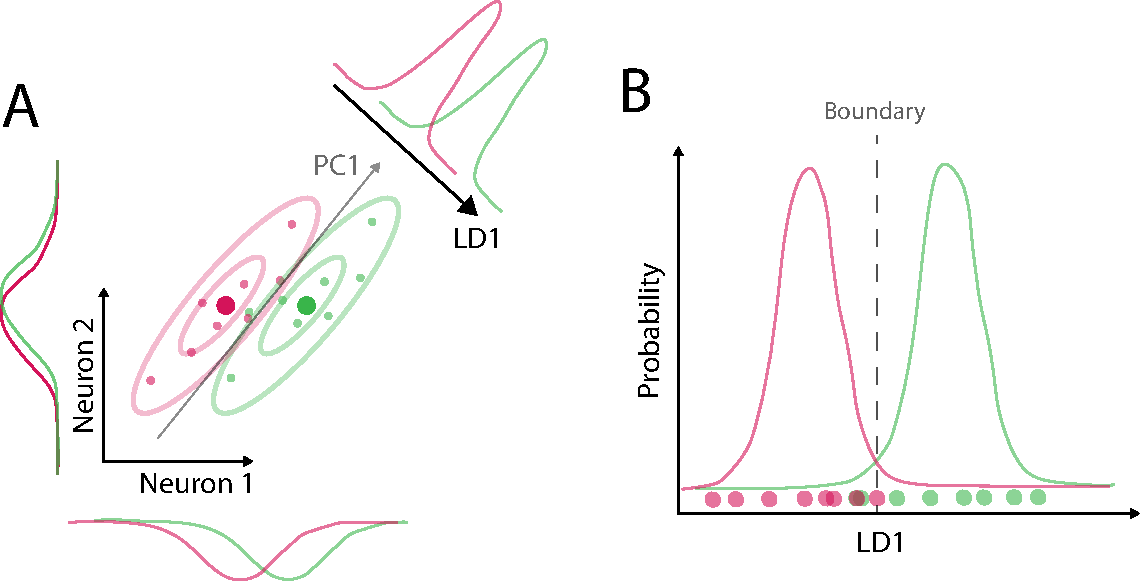
\includegraphics[width =  0.75\paperwidth]{Figures/R3_LDA_explaination.pdf}
       \caption[\label{fig:R3_F3} \textbf{Decoding using LDA}]{\label{fig:R3_F3} \textbf{Decoding using LDA. (A)} A schematic illustrating how LDA reduces dimensionally with respect to PCA given the activity of two neurons responding to two stimuli where stimulus identity is shown in red and green colors. The joint firing of the two neurons is overlapping in both the x and y axis. PCA would attempt to find the principal component that would preserve the maximum variance in the data (PC1). Instead LDA finds the projection of the data that maximises the distance between the means of the classes whilst minimising their scatter (known as the linear discriminant LD1). \textbf{(B)} Data in A projected into the 1D axis LD1. Both Gaussian are easier to separate in this projection. New test points can be classified by projecting them into this space and calculating the likely-hood that the point came from either Gaussian. The point is then assigned to the Gaussian that produced the greater likelihood. The decision boundary between the classes marks the point at which the probability of assignment to either Gaussian is 50\%.
    }
\end{figure}

\subsubsection{Logistic Regression}
\gls{logreg} unlike actual regression does not attempt to predict the numeric variable from a set of inputs. Instead, LogReg calculates the probability that a given input belongs to a certain class (only 2 classes are referred to here for simplicity) and finds a linear boundary that separates these classes. It does this by finding a weight vector $w$ that is orthogonal to this linear boundary such that when input $x$ is multiplied by this weight vector the output $z$, depending on its sign, denotes the class $Y$. Where positive values of $z$ indicate that a point lies above the decision boundary ($Y = 1$) and negative values indicate that the point lies below this decision boundary ($Y = 0$):

 \begin{equation}
    z(x) =  w_{1}x_{1} + w_{2}x_{2} + b     \begin{cases} 
      z < 0, & Y = 0\\
      z = 0,  & \text{x sits on the decision boundary}\\
      z < 0,  & Y = 1 \\ 
   \end{cases}
\end{equation}   

where $b$ is the lines intercept. However, to obtain the probability that x belongs to $Y$ this is fed into a logistic (or sigmoid) function $h(z)$:

\begin{equation}
    h(z) = \frac{1}{1 + e^{-z}}
\end{equation}

This function is takes values between 0 and 1 such that $h(z) = 0$ when $z$ goes to $-\infty$, and $h(z) = 1$ when z goes to $\infty$  and $h(z)$ = 0.5 when $z = 0$ (the decision boundary). Therefore $h(z)$ denotes the probability that Y = 1 and expresses the uncertainty of classifying points that are positioned closer to the decision boundary. This function can be fitted to a training data set by the cross entropy cost function: 

\begin{equation}
    J(h(z), Y) =  \frac{1}{n} \sum_{i = 1}^n Cost(h(z)_{i}, Y_{i})
\end{equation}

where:
\begin{equation}
    Cost(h(z), Y) =  -log(h(z)) & \text{,  if Y = 1}
\end{equation}

and:
\begin{equation}
    Cost(h(z), Y) =  -log(1 - h(z)) & \text{,  if Y = 0}
\end{equation}

As these functions are monotonically decreasing smooth functions they can be minimised using gradient descent, optimising the weight vector and maximising the likelihood of correct assignments. After estimating the parameters of the logistic function using training data the decoder can be used to predict the class of test data. Whilst only two dimensions and two classes are discussed here LogReg can be generalised to multidimensional multi-class problems. Unlike LDA, LogReg does not assume that the classes are normally distributed.

\subsubsection{Constructing population response vectors for decoder training and cross validation}
To train each decoder to predict the stimulus from tectal activity, the mean response for each neuron was calculated for each stimulus epoch. This gave a population response vector for each stimulus presentation in a Neuron x Epoch matrix and a corresponding label denoting the stimulus that elicited that response (\textbf{Figure \ref{fig:R3_F3}A}). The population responses and their corresponding labels were separated based on whether they occurred in an untextured or textured block so that decoding performance could be assessed for the blocks separately (\textbf{Figure \ref{fig:R3_F3}B}). To visualise how separable these population responses were, PCA was applied to these matrices. The transformed points were then plotted against the first two principal components and colored by their stimulus label with the point shape indicating the block. This revealed rough clustering of population responses to the 3 stimuli, indicating shared features between population responses that were evoked by the same stimulus (\textbf{Figure \ref{fig:R3_F3}C}). This indicates that there may be a degree of separability between these clusters that in principle could be well decoded by a linear decoder. However there was also some overlap between these clouds of points suggesting that there may be ambiguity in decoding stimulus identity. It is the extent of this overlap that is of interest because it may change with textured block or rearing condition. 

To assess decoding performance the decoders were trained on the majority of the data. However, each time the models were trained a single population response vector and its corresponding stimulus label were withheld for testing the trained models predictions.  The stimulus identity was then predicted using the trained model from this test point. This process was repeated so that every epoch was tested on once in a leave-one-out cross-validation strategy. The overall decoder performance was calculated as the number of correctly decoded stimuli as a percentage of all epochs tested. 

\subsection{Decoder performance in localising stimuli from tectal activity}
In the previous chapter, enriched fish consumed more prey when hunting over the GB whereas there was no change in the prey consumption of NR fish. One potential explanation for this is that the GR fish have learnt to use the contextual cues of the background to better locate the prey. Based on these results, it may be expected that the GR fish would show increased decoding performance when viewing the prey-like stimuli over the textured background whereas the NR fish would not. To test this, LogReg and LDA were used to decode stimuli from the 3 GR fish and 1 NR fish. To also test the effect of cells that were not responding to the stimulus on decoding performance this process was repeated for NCC cells and all cells (ie. NCC cells and non-NCC cells). This is because non-NCC cells are likely to reflect on-going tectal activity or behaviour and may fire sporadically, reducing decoding performance (\cite{Kahn2015ANeurons}). 

LogReg decoding performance was found to be tightly grouped between fish for both untextured and textured blocks when decoding from the NCC cells (\textbf{Figure \ref{fig:R3_F4}D}). For all GR fish decoding performance was higher in the textured block than the untextured block and appeared to be greater than the NR fish overall. Interestingly, the NR fish also showed a relatively large increase in decoding performance when viewing the stimuli over the textured background compared to the untextured background.  LogReg decoding on all cells resulted in variable decoding results and overall decoding performance was much lower than for the NCC neurons. Most fish (2 GR and 1 NR) still showed an increase in decoding performance in the textured block compared to the untextured block but 1 GR fish showed a decrease. Like LogReg, LDA decoding of NCC neurons also showed increases in decoding performance for most fish from untextured to textured blocks (\textbf{Figure \ref{fig:R3_F4}E}).  LDA decoding of all neurons however was highly variable between fish and was greatly reduced in general. Together these results suggest that fish may show an increased decoding performance when viewing stimuli over the textured background although more data is needed for the NR condition. In addition decoding from all cells together negatively impacts decoding performance overall, possibly due to cells that are not locked to the stimulus creating noise for the decoder. Therefore, to decode the stimulus location reliably from tectal activity only NCC neurons should be used.

Finally, to understand which decoder gave the best decoding performance the results for the NCC neurons for LDA and LogReg for the same fish and block were compared directly. This revealed that LogReg had the best decoding performance over all with an average increase of 5.2\% (p < 0.001, paired t-test) (\textbf{Figure \ref{fig:R3_F4}F}). This indicates that LogReg is the more powerful decoder in terms of segregating the population response space in these fish.


\begin{figure}[!ht]
        \captionsetup{}
        \centering
        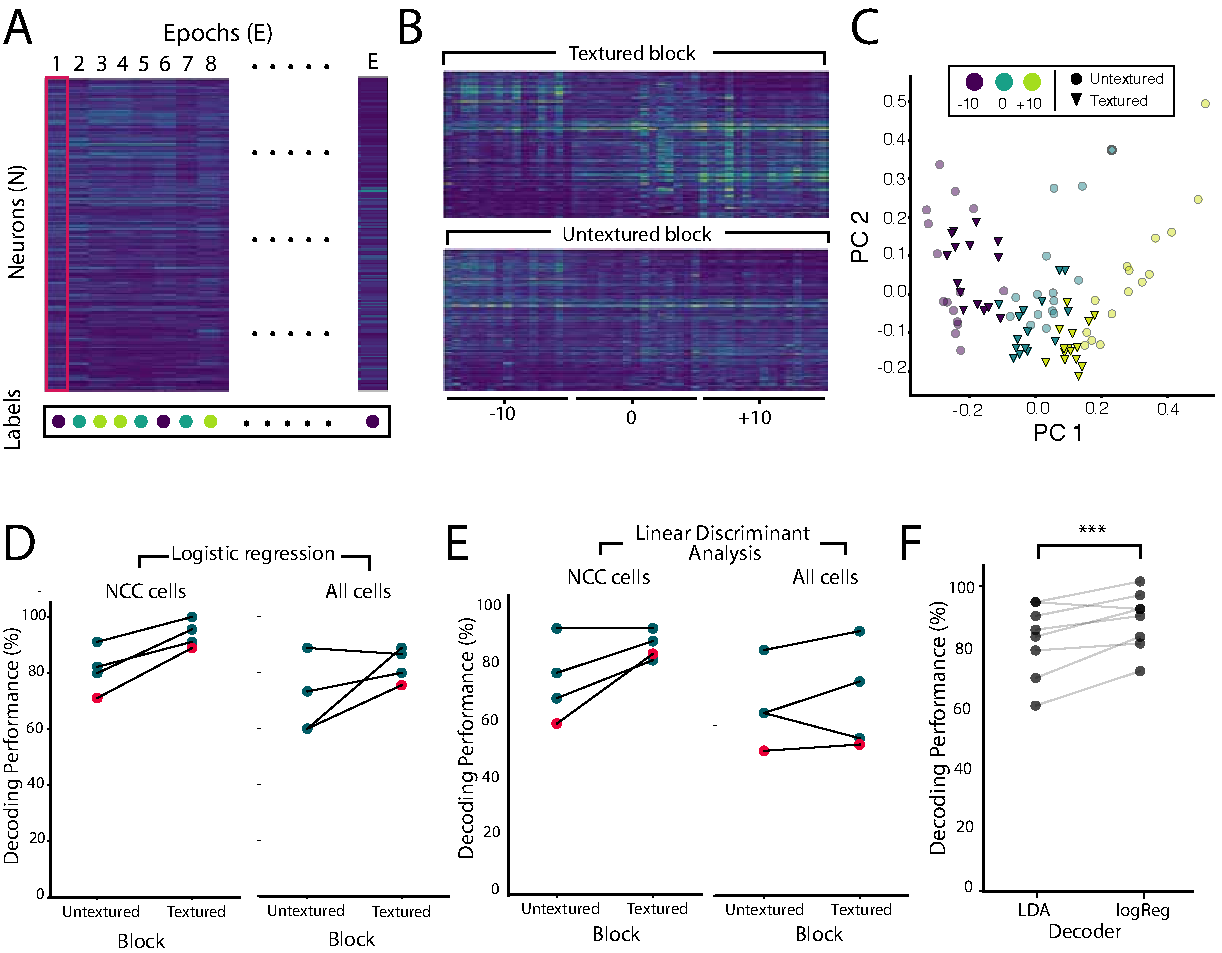
\includegraphics[width =  0.75\paperwidth]{Figures/Decoding_figure.pdf}
       \caption[\label{fig:R3_F4} \textbf{Decoding performance in classifying the position of the stimulus from tectal activity}]{\label{fig:R3_F4} \textbf{Decoding performance in classifying the position of the stimulus from tectal activity (A)}  To train the decoders the mean response for each neuron was calculated for each epoch. This gave a matrix of the dimensions (Neuron x Epoch) where each column represented a population response vector. For each population response vector there was corresponding label indicating the stimulus that caused it. \textbf{(B)} Population responses across stimulus repeats sorted by the stimulus that caused them for both the untextured and texutred blocks. \textbf{(C)} A PCA plot visualising population response vectors to each of the visual stimuli. Each point represents a single population response vector reduced to 2 dimensions (i.e the first two principle components - PC1, PC2). All population response vectors displayed are from a single fish. Colors indicate stimulus label and the shape of points denotes the block. \textbf{(D)} Decoding performance using \gls{logreg} to decode stimulus position during the two blocks for both NCC cells and all active cells. \textbf{(E)}  Decoding performance using LDA to decode stimulus position during the two blocks for both NCC cells and all active cells. \textbf{(F)} Comparing the performance of LDA and \gls{logreg} in decoding stimulus location from the same datasets (Untextured and textured blocks for NCC neurons in D). \gls{logreg} showed better decoding performance than LDA in all but one cases. *** = p < 0.001 .
    }
\end{figure}


\subsection{Population responses are more similar between stimulus locations in the textured block}
There are two possible reasons for the increased decoding performance when viewing stimuli over the textured background: 1) the similarity between population responses during stimulus repeats is decreasing when the fish are viewing stimuli over the untextured background, or 2) the population responses between stimuli at different locations are becoming more similar in the untextured block. A similarity index between a pair of vectors is defined by their normalized inner product, representing the cosine of the angle between two vectors:


\begin{equation}
    \cos(\theta) =  \frac{A\cdot B}{\|A\|\|B\|} = \frac{\sum_{i} A_{i} B_{i}}{\sqrt{\sum_{i}A_{i}^{2}} \sqrt{\sum_{i}B_{i}^{2}}}
\end{equation}


where $A$ and $B$ are vectors. If two population response vectors point to in the same direction in n dimensional space then they have a similarity index of 1. This would indicate that the exact same group of neurons are firing whereas a similarity index of 0 would indicate that the vector is orthogonal, with the two population vectors sharing no common neurons (\textbf{Figure \ref{fig:R3_F5}A}). Calculating the pairwise cosine similarity between all population response vectors and sorting them by the stimulus that caused them gives a matrix that makes it easy to visualise the similarity between stimulus repeats (close to the diagonal) and between different stimuli (off diagonal) (\textbf{Figure \ref{fig:R3_F5}B}). Doing this for the textured block reveals a discrete representation where there is high similarity within stimulus repeats but lower similarity between stimuli locations, particularly with those stimuli that are more distant in visual azimuth. For the untextured block this representation appears to far less discrete with increased off diagonal similarity between stimuli locations. To further visualise these differences in similarity between the two stimulus blocks sections of the matrix (denoted by white dotted lines in \textbf{Figure \ref{fig:R3_F5}B}) were averaged. This gave two 3 x 3 matrices where the diagonal represented the mean similarity between stimuli in the same location and the off diagonal values represented the mean similarity between different stimulus locations (\textbf{Figure \ref{fig:R3_F5}C}). Subtracting the averaged cosine similarity matrix for the untextured block from that of the textured block gave a difference in similarly matrix ($\Delta$ cosine similarity), allowing for changes in similarity to be visualised (\textbf{Figure \ref{fig:R3_F5}D}). All fish showed an increase in off diagonal similarity in the untextured block, particularly for stimuli that are further away. This result is consistent with the idea that the textured background may be contextually modifying tectal population activity, allowing for a more discrete representation of stimulus location. This could potentially explain the increased decoding performance for fish when viewing stimuli over the textured block.

\begin{figure}[!ht]
        \captionsetup{}
        \centering
        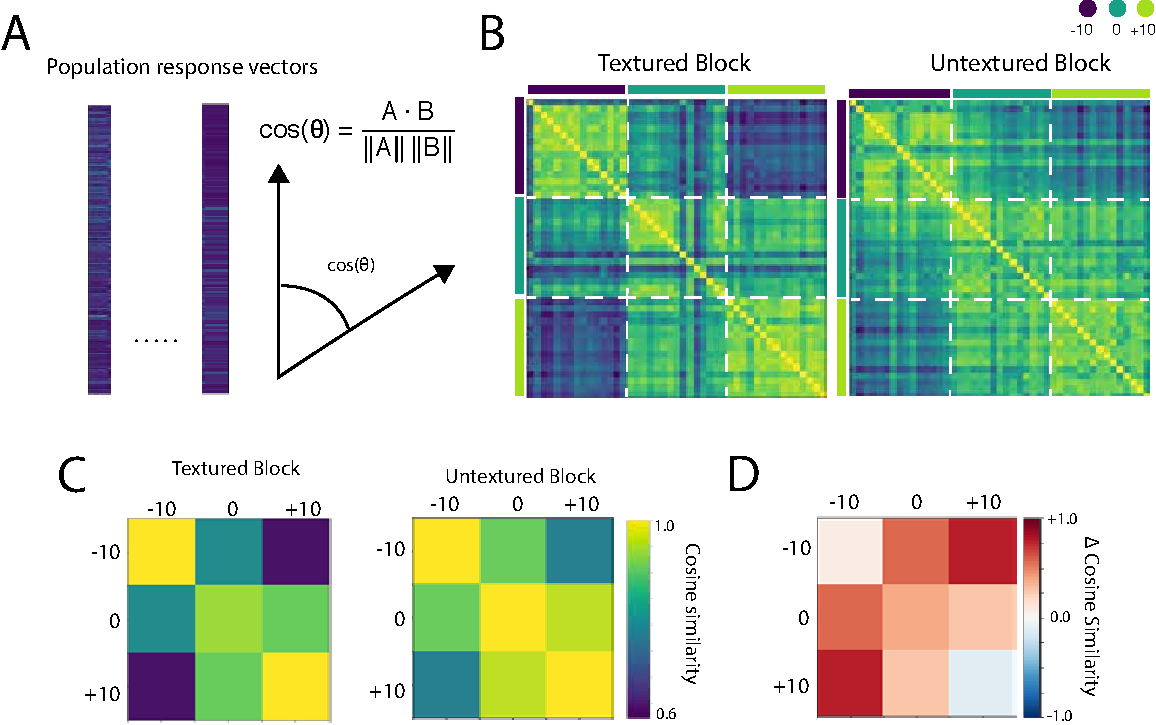
\includegraphics[width =  0.75\paperwidth]{Figures/R3_F3.pdf}
       \caption[\label{fig:R3_F5} \textbf{Decreased similarity between population responses for different stimuli in the textured block.}]{\label{fig:R3_F5} \textbf{Decreased similarity between population responses for different stimuli in the textured block. (A)} Population response vectors point to a location is response space. If two response vectors point to a similar point in space that means that they are similar in the responses that they contain. This degree of similarity can therefore be calculated by the cosine of the angle between the vectors given by the equation in A. As such a cosine similarity of 1 indicates that the vectors are pointing to the same point in space whereas 0 indicates that they are orthogonal \textbf{(B)} Cosine similarity matrices between population response vectors for the textured and untextured blocks. These have been sorted so that repeats of the same stimulus are neighbouring. This means makes is easy to visualise within stimulus location similarity (close to the diagonal) and between stimulus location similarity (off diagonal). This reveals that when viewing stimuli over the textured background there appears to be decreased similarity between population response compeared to the untextured block. \textbf{(C)} Averaging together the the regions outlined by the dotted lines in B gives a mean summary value for both with stimulus and between stimuli similarities. \textbf{(D)} Taking the difference between the mean similarity matrices gives the difference in cosine similarity ($\Delta$ Cosine similarity). This shows that there is increased similarity between stimulus further away from each other in visual azimuth.  
    }
\end{figure}



\subsection{Tracking and analysing tail movements}
In addition to being able to monitor neural activity, the virtual reality hunting setup also allows for the tail movement of the fish to be monitored using a high speed camera positioned below the imaging chamber. This allows difference in the ability of the prey-like stimuli to induce tail movements as a result of the textured blocks or rearing conditions to be examined. Changes in this ability may indicate a difference in the larvae's detection or perception of prey. The tail movements for only 1 GR fish have been recorded during visual stimulation. However, the following section outlines the pipeline I have developed to analyse this behavioural data.

Accurate quantification of tail motion requires regions of the tail to be tracked. This was achieved by training a \gls{cnn} to recognise equally spaced points along the tail length.  The CNN was implemented using \gls{dlc} (\cite{Mathis2018DeepLabCut:Learning}) (see \textbf{Materials and methods}). To train \gls{dlc} 250 frames from 3 separate tail recordings of spontaneous tail movement were manually labeled. 200 of these frames were used to train the model and 50 were used as a test dataset to evaluate the model performance. This showed that the mean error between predicted labels and manual labels was around 8 pixels. As the width of the tail is around 13 pixels this error was deemed to be acceptable for accurate tracking of tail position. Furthermore, visual inspection of the videos with the predicted markers overlayed revealed that the model tracked the extent of tail well (\textbf{Figure \ref{fig:R3_F6}A}). However, on some high velocity tail movements the tail tip was incorrectly assigned to regions of high luminance in the background caused by infrared light reflections from the microscope objective. This is likely to be due to the poor contrast between the tail tip and background.

To compute a behavioural trace the tail was skeletonized by treating the regions between the markers as separate vectors (bones). The angle of each of these bones relative to the midline was calculated and summed to give the total tail angle. This measure of tail angle is centered at zero when the tail is in line with the body axis and negative deflections indicate tail movements toward the stimulus (\textbf{Figure \ref{fig:R3_F6}B-D)}.  As previously reported head fixed fish were found to move in brief swim bouts with longer inter-bout intervals (\cite{Semmelhack2014}). These bouts could be automatically detected by taking the absolute value of the first derivative of the tail angle trace. Smoothing this trace with a Guassian kernel had the effect of dilating neighbouring tail beats and joining them together. This could then be threshold to each segmented swim bout  (\textbf{Figure \ref{fig:R3_F6}E}) (see \textbf{Materials and methods} for details).

For the one imaged GR fish the likelihood of the tail moving within an epoch was low with only 7.7\% of epochs containing a movement. Whilst this is insufficient data to compare between conditions there are a number of metrics that could be extracted from these within epoch movements including: 1) the probability that the stimulus elicits a tail movement, 2) the latency between stimulus onset and tail movement, 3) the tail angle of the first turn 4) whether this turn was towards the stimulus (\textbf{Figure \ref{fig:R3_F6}F}). Interestingly for the single imaged fish the first turn for all within epoch movements were in the direction of the stimulus, potentially indicating approach behaviours. 

\begin{figure}[!ht]
        \captionsetup{}
        \centering
        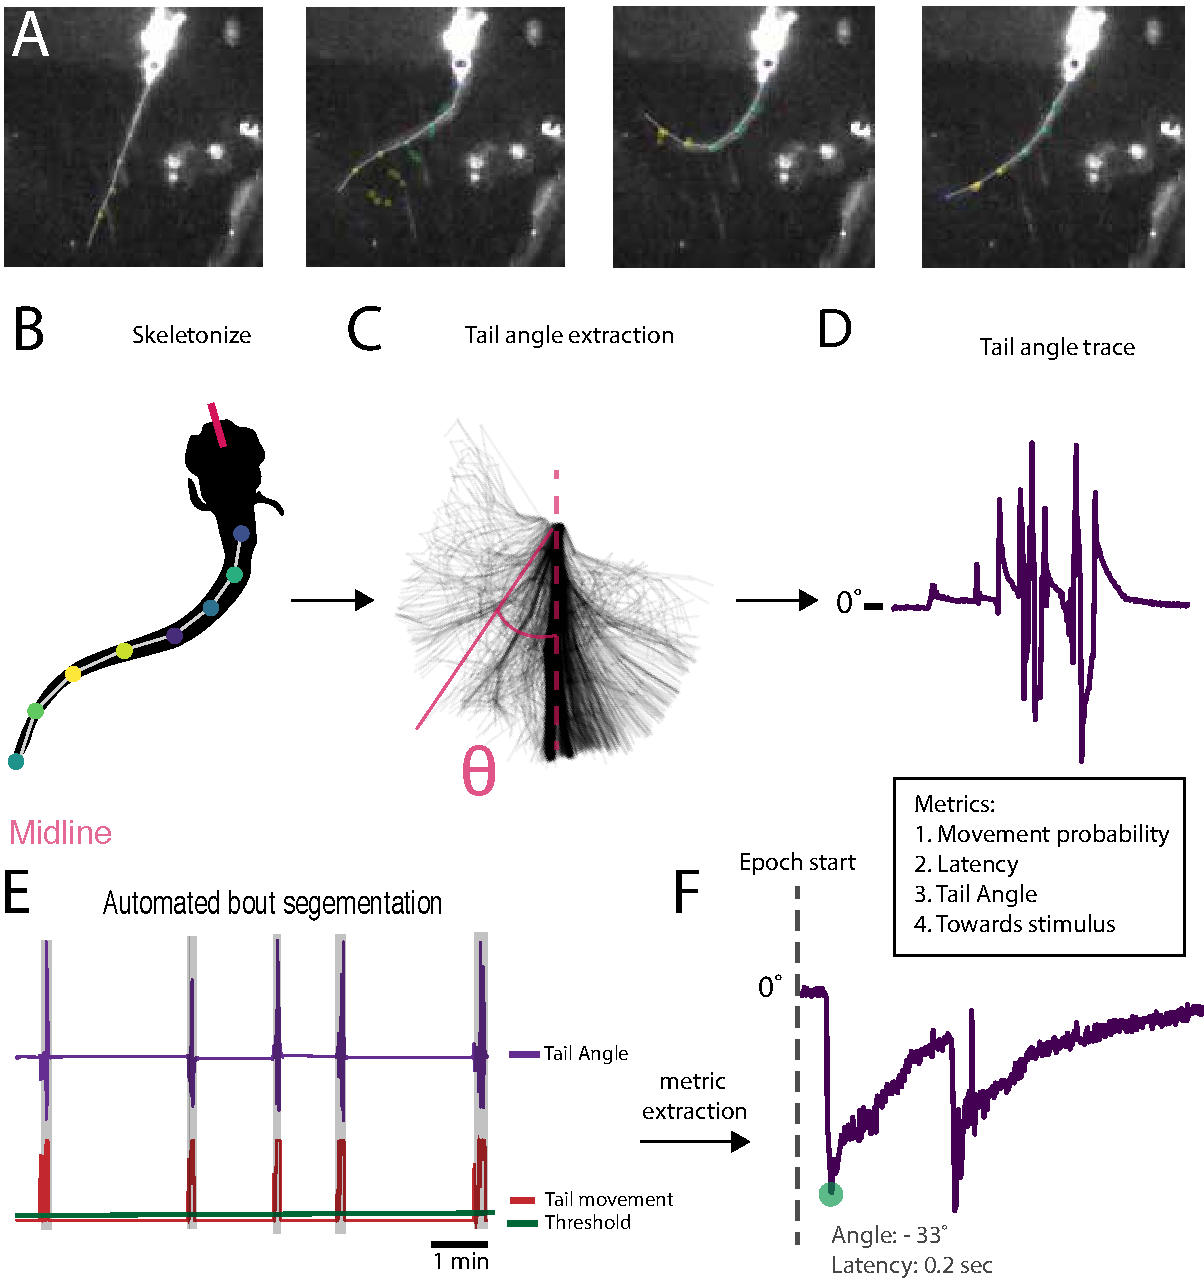
\includegraphics[width =  0.7\paperwidth]{Figures/R3_F4.pdf}
       \caption[\label{fig:R3_F6} \textbf{Tracking and analysis of tail movements in head fished larvae.}]{\label{fig:R3_F6} \textbf{Tracking and analysis of tail movements in head fished larvae. (A)} Tail movements were imaged using a high speed camera recording at 450Hz. The tail could then be tracked using a CNN (implemented in DLC) trained on 200 frames extracted from tail recordings of different fish. These images show the tracking of the tail during a single swim bout. Dots show the position of the labelled markers which have been joined with a skeleton of lines between the markers. Markers in these images also show the "trails" of the markers in the previous 3 frames. \textbf{(B)} Schematic showing the position of the eight markers along the tail and the bones of the skeleton in between. \textbf{(C)} A maximum projection of the skeletonized fish tail in a single bout of movement. The tail angle was calculated as the sum of the angles of each bone of the skeleton deviating from the midline. \textbf{(D)}  This gave a behavioural trace representing the tail angle. Here is an example of that trace during one bout of tail movement. \textbf{(E)} Tail movement bouts were detected by calculating the first derivative of the tail angle (purple) and smoothing it with a Gaussian kernel (tail movement trace in red). This had the effect of dilating neighbouring tail beats and joins them together so that they can be segmented using a threshold (green). This allows for each bout to be automatically detected (shaded grey areas). \textbf{(F)} Metrics for bouts occurring within a stimulus epoch can then be estimated. These metrics will include 1) the probability of tail movement, 2) the latency of movement relative to stimulus onset, 3) Tail angle of the first tail movement and 4) whether the movement was towards the stimulus or not. These metrics will allow for the ability of the prey-like stimuli to induce prey-like stimuli to be examined.
       }
\end{figure}

\section{Discussion}
In the previous chapter GR fish were found to consume more prey specifically when hunting over the GB, suggesting a context specific change in their ability to hunt prey. To investigate this hypothesis a virtual reality hunting assay was developed which allowed for simultaneous recording of tectal activity and tail movements while prey-like stimuli were presented at different positions in visual azimuth. Importantly, these stimuli were presented over either an untextured or textured background mimicking the differences in the visual environment in the freely swimming hunting assay.  To understand if the sensory representation of prey location was contextually modulated by the background the position of the stimulus was decoded from visually evoked tectal activity using different decoding methods. This showed that position of the prey-like stimulus could be most accurately decoded from tectal activity using \gls{logreg} and that all fish showed an improvement in decoding performance when viewing the stimulus over the textured background. This preliminary data suggests that population responses in the tectum may be contextually modulated by the textured background to give a more accurate encoding of stimulus position. Finally, tail movements can also be monitored and tracked allowing for accurate quantification of stimulus induced swimming bouts. Therefore this experimental assay could be used in future work to understand how tectal activity and behaviour are modulated by the context of the background.

\subsection{Decoding stimulus location from tectal activity}
Decoding performance is likely to be affected by the choice of decoder and may lead to poor results, or conclusions from changes in decoding performance, if an inadequate decoder is used. Therefore the decoder must be able to decode the stimulus accurately and any changes in decoding performance should also be predictive of changes in behaviour.  As the tectum exhibits a topographic map of visual space it may be expected that stimulus position could be accurately decoded from the position of responding neurons within the tectum. However, while the the tectal topographic map is linear and smooth at the macroscale at the local level it is very imprecise containing a significant number of misplaced cells (\cite{Niell2005FunctionalTectum}; \cite{Romano2017}). This imprecision leads to very poor decoding performance when using topographic decoders (\cite{Avitan2016}). In contrast, statistically optimal decoders such as a maximum likelihood decoders have been found to decode stimulus location from tectal activity with very high performance. Maximum likelihood decoders estimate the statistically most likely stimulus to cause a population response. This is calculated using the full distribution over each neurons response to each stimulus repeat. Whilst a biologically plausible implementation of maximum likelihood decoders has been suggested (\cite{Jazayeri2006OptimalPopulations}) similar decoding performance can also be achieved through linear decoders such as LDA (\cite{Avitan2016}; \cite{Avitan2019}). However, linear decoders are far simpler in their implementation than maximum likelihood decoders and may be closer to the types of computations that are actually performed in the nervous system (\cite{Salinas1994VectorRates}). In addition, linear decoders have recently been used to examine how the tectal representation of stimulus position refines over development (\cite{Avitan2019}). This showed that decoding performance in the regions of the tectum dedicated to the stimuli in the frontal visual field improved correlating with improved prey detection within this region as hunting develops. Furthermore, by performing decoding alongside hunting assays in the same fish showed that decoding performance was predictive of hunting performance at the level of individual fish. While it is not clear how the tectum actually decodes stimulus location, these results show that changes in linear decoding performance are relevant to changes in hunting performance. 

In this chapter I used two linear decoders to predict stimulus position from tectal activity. The reason for doing this was firstly to ensure that changes in decoding performance were not an artifact of using a specific decoder and secondly because the previously used LDA decoder assumes that the data is normally distributed. As a result any changes in decoding performance may be related to violations of this assumption rather than a difference in the tectums ability to localise a stimulus. Therefore in addition to LDA a LogReg decoder was also used as it does not make this assumption. While these decoders were broadly in agreement LogReg had increased decoding performance compeared to LDA in nearly all cases, suggesting that LogReg is better at separating the population response space. This increased performance may reflect that the underlying distribution of population responses are not normally distributed.

Another factor that is likely to affect affect decoding performance is what cells are used for the decoding. For example, while some neurons had a firing patterns that were locked to the stimulus, a larger proportion of tectal neurons did not appear to show visually evoked activity. These neurons, which fire sporadically, are likely to reflect ongoing activity and activity related to behaviour. This sporadic activity, particularly when the training dataset size is small, could negatively impact decoding performance by creating noise (\cite{Kahn2015ANeurons}). To assess the impact of these cells on the ability to decode stimulus location an NCC measure was calculated for each cell and compeared to its own randomly firing null model. This allowed neurons that were responding to the stimulus (NCC cells) to be distinguished from those that were firing more randomly relative to the stimulus (non-NCC cells). Decoding either all tectal cells (NCC and non-NCC cells) or from the NCC cells alone revealed that decoding performance was impacted by ongoing activity in the non-NCC cells. This also increased the variability in decoding performance between fish. Therefore decoding in future experiments should be performed on the NCC neurons alone, as these are the neurons that carry information that is relevant for the task.

\subsection{Contextual modulation of the tectal representation of stimulus location.}

The results from the behavioural assay in Chapter 4 suggest that enriched fish may be learning to use the background to either better detect or locate the prey, leading to higher prey consumption when hunting over the GB. If this is the case it is predicted that decoding performance should be higher when enriched fish view prey over the textured background. By decoding the stimulus location from visually responsive neurons revealed an increase in decoding performance for the GR reared fish when viewing prey-like stimuli over the textured background. This suggests that the tectum is may be encoding more information about the location of each stimulus specifically in the textured block. Furthermore, population responses evoked by stimuli in different locations were found to be less similar when the fish viewed the stimuli over the textured background, leading to a more discrete representation of stimulus location and potentially accounting for the change in decoding performance. Together these results suggest that the representation of the stimuli may be modulated by the context of the background and may allow the fish to better locate prey against textured background.

While these experiments show that there is a clear difference in the population response responses between untextured and textured blocks it is not yet clear what specific features of population activity may be altered to bring about these differences in decoding performance.  However, it is well known that the tuning properties of neurons are not fixed. Instead they can be modulated by features in the visual scene presented outside of the neurons receptive field in multiple species and at different stages of the the visual system (\cite{Krause2014ContextualCortex,Allman1985StimulusNeurons}). This demonstrates that response to a stimulus can be dependent on the context within which the stimulus is presented.  For example, in the optic tectum of pigeons and retina of mice the response of certain direction selective neurons can be influenced by the direction global motion outside of the receptive field location. This suggests that these neurons may be able to distinguish between self motion and local object motion (\cite{Sun2002ContextualPigeons, Sun2006ONRetina}).  Alternatively, other tuning properties such as size and contrast can also be influenced by context (\cite{Krause2014ContextualCortex, Ziemba2018ContextualV2}). Furthermore, identifying salient stimuli such as a vertical bar in a sea of horizontal bars is thought to rely on a mechanism "isofeature" suppression (\cite{Zhaoping2016FromNeuroscience}). Within this mechanism neurons responding to the same/similar features (such as the horizontal bars) tend to suppress each other whereas neurons responding to the different feature (the vertical bar) escape this suppression and fire with higher amplitude.  This leads to a winner take all computation where attention is diverted to the location of the stimulus eliciting the greatest response in both the visual cortex of primates (\cite{Zhaoping2012PropertiesBehavior}; \cite{Allman1985StimulusNeurons}) and the optic tectum of archerfish (\cite{Ben-Tov2015Pop-outFish}).  Such mechanisms of contextual modulation may be important for processing natural visual scenes where salient features such as prey are seldom found in isolation.  Instead natural visual scenes are cluttered with an array of different visual features that need to be perceptually segmented from the salient feature (\cite{Zhaoping2016FromNeuroscience}). Therefore contextual modulation of receptive fields may be important for for identifying prey against the textured background. 

In these current experiments there are a number of features that could be modulated by the presence of the background leading to changes in decoding performance. Firstly, it is possible that the spatial tuning of neurons responding to prey-like stimuli may be sharpened by the context of the textured background. This could lead to decreased similarity between populations responses for the different stimuli in the textured block. To investigate this future experiments could include a larger number of stimulus locations. This would allow for a Gaussian to be fitted to the average response to each stimulus position for a neuron to give a tuning curve. Doing this separately for the textured and untextured block would reveal if the tuning of tectal neurons is changing contextually with the change in background. Alternatively, it could be that the relative motion of the stimulus against the textured background maximally stimulates tectal neurons or that a suppression mechanism from features responding to similar stimuli restricts the spatial spread of responses. Both of which could lead to decreased similarity between population responses in the textured block. These hypotheses could be investigated in future studies either by changing stimulus parameters or by closer inspection of how tectal responses are changing between the two blocks.

 It is possible that contextual modulation of tectal responses is something that is learnt through experience, if this is true then the NR fish should not show increased decoding performance when viewing the stimuli over the textured block. Despite the GR fish showing increased decoding performance overall, the one NR fish that was imaged also showed a increase in decoding performance when viewing stimuli over the textured background. As this is only one fish more data is needed to understand if this decoding performance is also dependent on rearing condition. However, if this result is consistent it would be unclear how this change in decoding performance between the two blocks relates to the increased prey consumption of enriched fish when hunting over the GB and may indicate. This highlights the difficulty of being able to relate changes in the brain to behaviour. Ideally future experiments would use the the same animal for the freely swimming hunting assay and virtual hunting experiments in order to relate changes in the the tectum to hunting performance (\cite{Avitan2019}). Either the overall decoding performance, or the changes in decoding performance between the two blocks, could be correlated with changes in prey consumption at the level of individual fish. This would allow which features may be relevant to the behaviour to be identified.
 
\subsection{Monitoring tail movements within the virtual reality setup}
Head fixed zebrafish larvae are known to respond to prey-like stimuli with movements that are characteristic of hunting (\cite{Bianco2011}; \cite{Bianco2015}; \cite{Semmelhack2014}). These include small unilateral bends of the tail tip towards the stimulus location known as J-turns which, in freely swimming fish, orientate the fish towards the prey. Monitoring these tail movements could potentially allow for the differences in the ability of prey-like stimuli in driving behaviour to be examined when these fish view them over the textured and untextured backgrounds. Such differences would indicate a difference in the ability of these fish to detect or perceive the prey within the context of the background that could potentially lead to increased prey consumption in the freely swimming hunting assay. Therefore tail movements were then tracked using \gls{dlc} giving accurate quantification of the tail kinematics at multiple points along the tail. As in previous studies the one imaged fish in this chapter appeared to move in discrete bouts followed by long inter-bout intervals making them easy to segment (\cite{Semmelhack2014}).  The probability of the fish moving within an epoch was found to be low at around 7 \%. However, this is actually comparable to some other studies with even the most optimal stimuli in one study eliciting hunting behaviours in  5-10 \% of stimulus presentations (\cite{Bianco2015}). It was difficult to see if these movements resembled the J-turns that are known to orientate the fish toward the prey. This may reflect the fact that previous studies have used spots that move across the whole visual field rather than a spot moving within a local neighbourhood and therefore the degree to which the animal needs to turn may be different (\cite{Bianco2011}; \cite{Bianco2015}, \cite{Semmelhack2014}; \cite{Jouary2016ALarvae}). Despite this, all within epoch tail movements in the GR fish were found to elicit tail movements towards the side that the stimulus was being presented. This suggests that they may represent the intent of the fish to approach the stimulus. 

One way to understand if these within epoch movements are related to the initiation of hunting is to also free the eyes of the fish and track their movement (\cite{Bianco2015}). This is because eye convergence only occurs at the initiation of hunting as opposed more ambiguous tail movements which may be related to either hunting, spontaneous swims or struggles in the agarose (\cite{Bianco2015}; \cite{Semmelhack2014}). During decoding experiments the eye position needs to be fixed so that the same region of the retina can be reliably stimulated. However, eye convergence could be used to identify coincident tail movements that may related to hunting in preparations where the eyes are free. Paramaterising these tail bouts using metrics such tail angle, tail beat frequency and bout duration could be used to train a classifier that could distinguish between spontaneous swims and hunting turns. This classifier could then be used to identify J-turns that occur when the eyes are fixed for decoding experiments, similar classifiers have previously been used for the automatic identification of prey capture swims (\cite{Semmelhack2014}). With more data for both GR and NR fish it would be interesting to understand if tail movements differ between the rearing conditions such as the probability that a stimulus causes a prey capture swim or if the latency of the swim changes relative to the stimulus on set. These may indicate a difference in the ability of these fish to detect or perceive the prey-like stimuli, potentially allowing GR fish to engage in hunting episodes with a higher frequency relative to NR fish. 

In summary, this chapter outlines an experimental protocol that could be used to understand how the tectum responds differently to prey-like stimuli when they are presented over different backgrounds. This can be viewed alongside the ability of these stimuli to cause tail movements. Preliminary results suggest that all fish show increased decoding performance when viewing the stimuli over the textured background, suggesting that tectal responses may be contextually modulated. Collecting more data in future experiments may reveal differences between GR and NR fish in how they respond to these prey-like stimuli. This may explain the differences in prey consumption that were observed in chapter 4.



